\documentclass[12pt,a4paper]{report}
\usepackage[utf8]{inputenc}
\usepackage{amsmath}
\usepackage{amsfonts}
\usepackage{amssymb}
\usepackage{graphicx}
\usepackage{caption}
\usepackage{svg}
%\usepackage{gensymb}
\usepackage{fourier}
\usepackage[francais]{babel}
\usepackage{eurosym}

\usepackage[top=2.5cm,bottom=2.5cm,right=2.5cm,left=2.5cm]{geometry}

\usepackage{url}
\usepackage{moreverb}
%\usepackage{multirow}
%\author{LEJEUNE Raphaël}
%\title{Titre}

\usepackage[fpms]{umons-coverpage}
\umonsAuthor{Raphaël \textsc{LEJEUNE} \\ Maximilien \textsc{POTTIEZ}}
\umonsTitle{Un robot contrôlé via un Raspberry Pi}
\umonsSubtitle{Projet d'informatique}
\umonsDocumentType{Rapport de projet}
\umonsSupervisor{Sous la direction de Monsieur le Professeur\\ Mohammed \textsc{BENJELLOUN}}
\umonsDate{2015}

\begin{document}

\umonsCoverPage

\tableofcontents

\chapter{Introduction}

Décrire le but visé, l'utilité du robot.

Faire en français et en anglais !

\begin{figure}[hf!]
\center
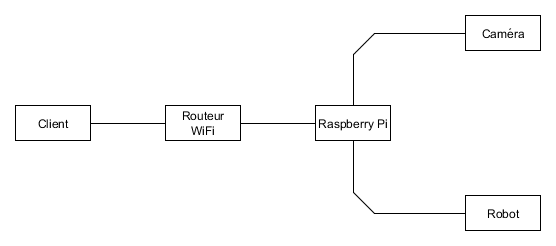
\includegraphics[scale=0.6]{images/GraphMateriel.png}
\caption{Matériel}
\end{figure}

\chapter{Matériel} \label{Matériel}

%Lister le matériel utilisé, justifier sa présence
%
%- Raspberry (pourquoi pas un Arduino, par exemple ?)
%- Moteurs (quel modèle ?)
%- Contrôleur (expliquer son utilité)
%- Batterie
%- Clé wifi
%- Webcam (caractéristiques techniques)
%- Réseau Wi-Fi opérationnel
%- ?

Voici la liste complète du matériel que nous avons utilisé :

\paragraph{Kit} Le kit que nous utilisons se compose des éléments suivants :

\begin{itemize}
\item Chassis Bundle
\item Raspberry pi 2
\item Arduino
\item Batterie : TeckNet iEP387
\item Carte micro SD
\item Raspberry pi camera
\item Wifi : Edimax EW-7811Un -150Mbps
\end{itemize}

\begin{figure}[hf!]
\center
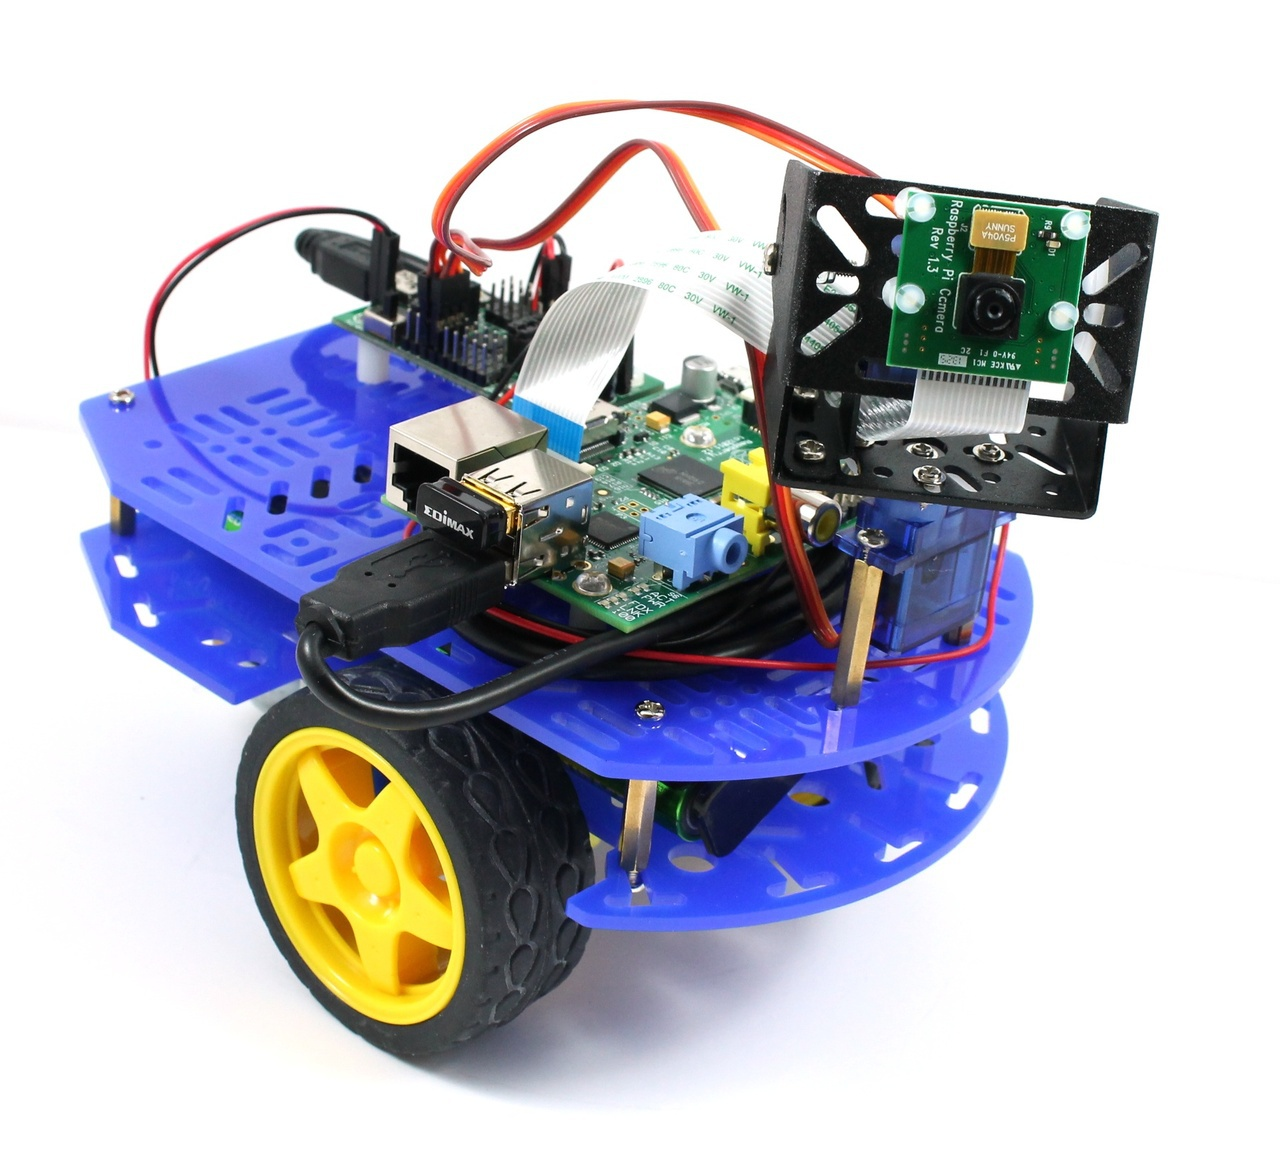
\includegraphics[scale=0.2]{images/kit.jpg}
\caption{Robot complet}
\end{figure}

\paragraph{Raspberry Pi} Nous avons donc utilisé deux modèles de raspberry pi lors de notre projet le Raspberry Pi B+ et le Raspberry Pi 2. 
Bien que visuellement, ces deux modèles se ressemblent très fort, leurs caractéristiques sont différentes :

\begin{tabular}{l|p{4.5 cm}|p{4.5 cm}}
 & Modèle B+ & Modèle 2 \\ 
\hline 
Mémoire RAM & 512 Mo & 1 Go \\ 
Processeur & ARMv6 & ARMv7 (4 coeurs) \\
Fréquence du processeur & 700 MHz & 900 MHz \\
Mémoire de stockage & MicroSD & MicroSD \\
Ports & 4 USB 2.0, HDMI, RJ45 \newline Jack (3.5mm), 40 broches GPIO & 4 USB 2.0, HDMI, RJ45, Jack (3.5mm), 40 broches GPIO \\
Consommation & 600 mA, 3.5 W & 600 mA, 3.5 W \\
Prix & environ 30 \euro & environ 40 \euro \\
Système d'exploitation & Linux & Linux, ou Windows 10
\end{tabular}

\begin{figure}[htbp]
\begin{minipage}[c]{.45\linewidth}
\begin{center}
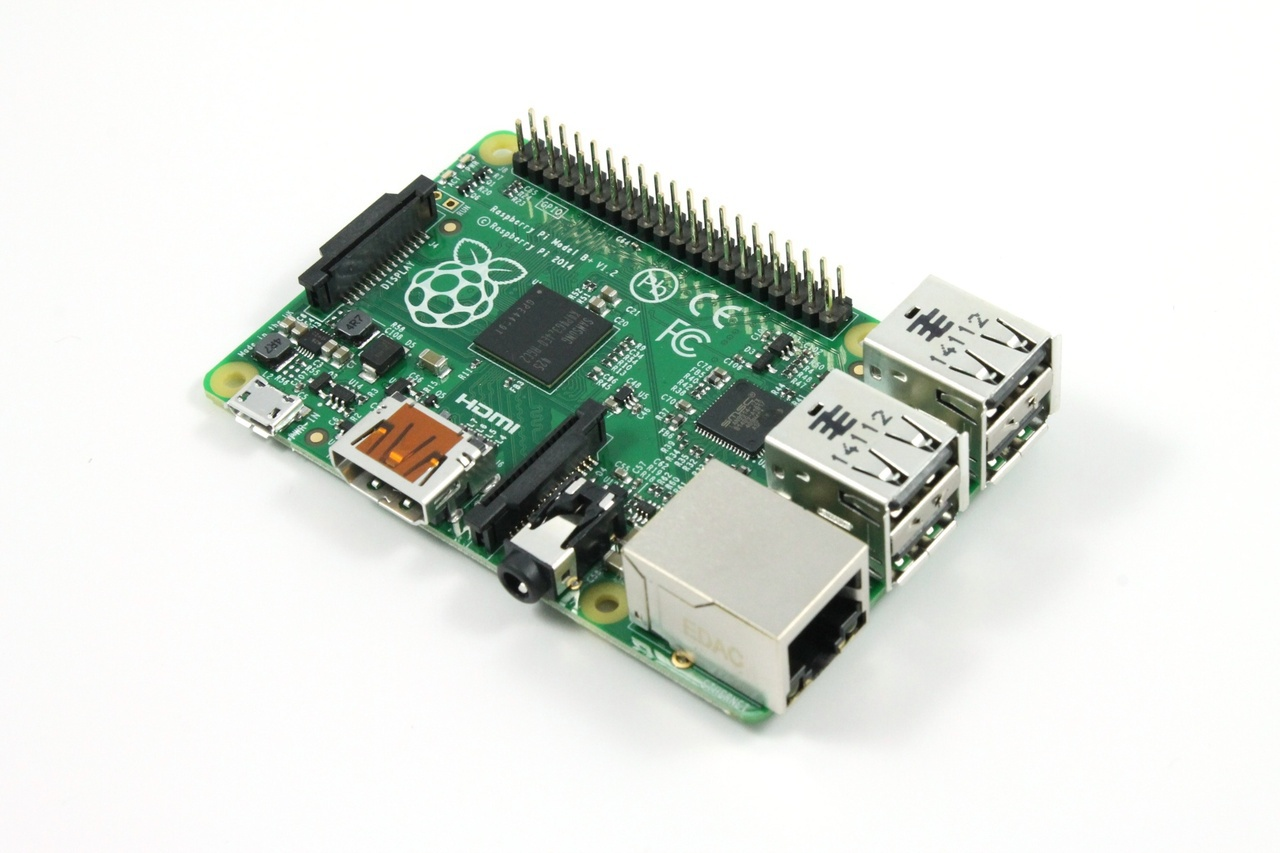
\includegraphics[scale=0.2]{images/modelB+.jpg}
\caption{Raspberry Pi B+}
%\label{}
\end{center}
\end{minipage}
\hfill
\begin{minipage}[c]{.45\linewidth}
\begin{center}
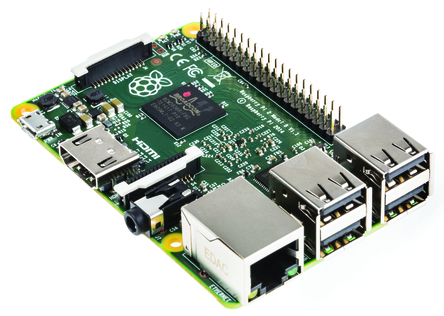
\includegraphics[scale=0.4]{images/model2.jpg}
\caption{Raspberry Pi 2}
%\label{}
\end{center}
\end{minipage}
\end{figure}

\paragraph{Arduino} C'est la carte Arduino qui fait le lien entre le Raspberry et les moteurs. Nous avons testé deux modèles différents :

\begin{tabular}{l|p{4.5 cm}|p{4.5 cm}}
 & Dagu mini driver & Dagu mini driver MKII \\ 
\hline 
Processeur & ATMega8A & ATMega328P \\
Fréquence du processeur & 16 MHz & 16 MHz \\
Prix & environ 10 \euro & environ 12 \euro \\
\end{tabular}

\begin{figure}[htbp]
\begin{minipage}[c]{.45\linewidth}
\begin{center}
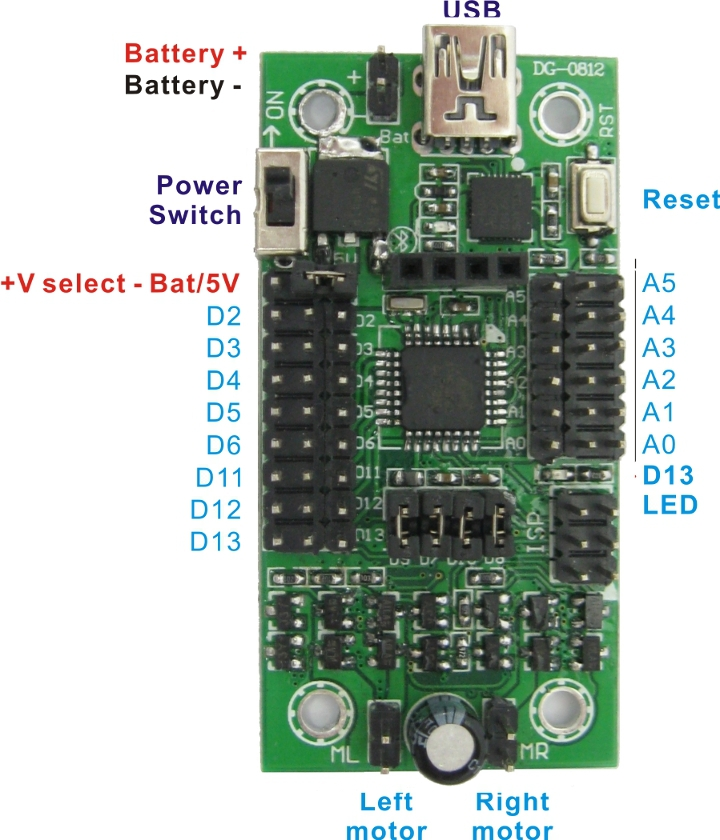
\includegraphics[scale=0.5]{images/mini_driver.jpg}
\caption{Dagu mini driver}
%\label{}
\end{center}
\end{minipage}
\hfill
\begin{minipage}[c]{.45\linewidth}
\begin{center}
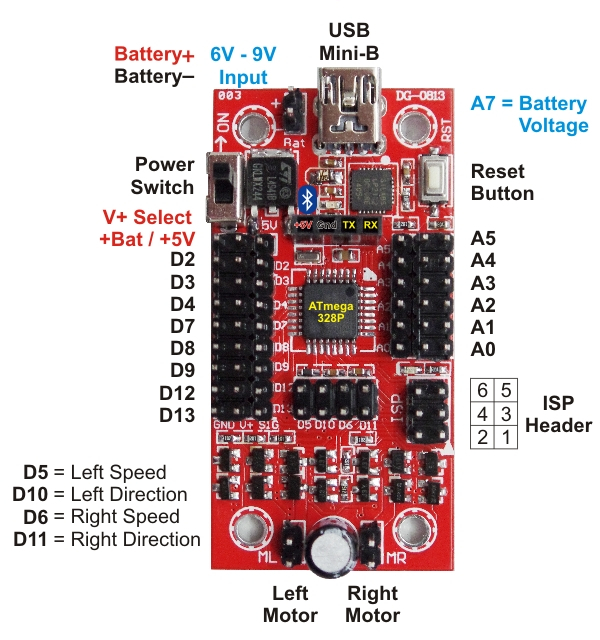
\includegraphics[scale=1]{images/Mini_Driver_MkII.jpg}
\caption{Dagu mini driver MKII}
%\label{}
\end{center}
\end{minipage}
\end{figure}

%\chapter{Software}
%
%%Trouver un autre titre !!!
%
%%Ici expliquer le principe des signaux PWM, des sockets, du multi-thread (même si pas utilisé... Parler des pistes envisagées)
%
%%Captures d'écran
%
%Lors de la réalisation du projet, nous avons envisagé plusieurs pistes pour contrôler le robot. 
%
%\section{Signaux PWM}
%
%Pour contrôler les moteurs, nous pouvons utiliser les signaux PWM (\textit{Pulse Width Modulation}) : il s'agit d'ondes carrées périodiques. 
%
%Pour chaque période, on envoie une tension continue de 5 volts (qui correspond à la tension de base du Raspberry Pi, délivrée sur les ports GPIO) pendant une fraction de la période seulement. La tension « perçue » par le moteur est directement proportionnelle à cette fraction. Si cette fraction vaut par exemple 60 \%, le moteur tournera comme si on envoyait 3 V, donc à 60 \% de son régime maximum, si sa tension nominale est de 5 V. 

\chapter{Organisation}

\begin{figure}[hf!]
\center
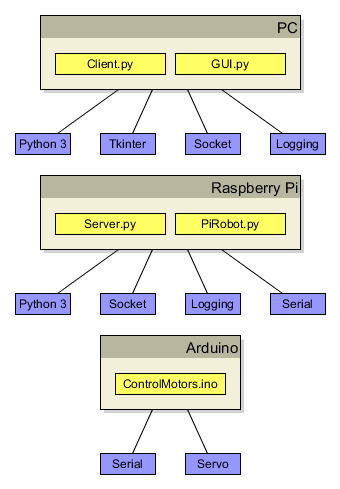
\includegraphics[scale=0.6]{images/GraphLogiciel.png}
\caption{Logiciel}
\end{figure}

Notre code est divisé en trois parties :

\bigbreak

\begin{itemize}
\item La partie client, qui tourne sur un PC (sous Windows, Linux, ...),
\item La partie serveur, qui se trouve sur le Raspberry Pi,
\item La partie contrôle, qui se trouve sur la carte Arduino.
\end{itemize}

\bigbreak

\paragraph{Client.py} sert à communiquer avec le Raspberry Pi. C'est dans ce fichier que sont récupérées toutes les requêtes de l'utilisateur, lorsqu'il appuie sur un bouton, par exemple.

\paragraph{GUI.py} sert à tracer l'interface graphique. Nous avons voulu créer des fonctions dans ce fichier et les lier directement au bouton comme ci-après :

\begin{verbatimtab}[3]
buttonstop = Button(frameRoot, text="STOP", command=buttonstopclick)
\end{verbatimtab}

Mais cela a entraîné des erreurs de références circulaires (car \textit{Client.py} dépend de \textit{GUI.py} et \textit{GUI.py} dépend de \textit{Client.py}). Nous avons résolu ce problème en ne donnant pas de fonction au bouton. Dans \textit{Client.py}, nous donnons explicitement la commande suivante :

\begin{verbatimtab}[3]
GUI.buttonstop.bind("<Button-1>", buttonstopclick)
\end{verbatimtab}

Cette seconde option présente deux avantages : on peut choisir le type d'événement à associer (bouton cliqué ou relâché, ...), et on peut aussi supprimer ce lien (avec la commande \verb=unbind=).

\paragraph{Server.py} est le programme qui tourne sur le Raspberry Pi. Son but est de recevoir les messages (depuis le client) et de les interpréter pour envoyer des instructions au robot.

\paragraph{PiRobot.py} est une classe qui contient toutes les fonctions d'envoi de commandes au robot, ainsi quand \textit{Server.py} reçoit un message, il n'a qu'à appeler la bonne fonction (par exemple la fonction \verb=Stop=, qui envoie une commande au robot pour arrêter les moteurs).

\paragraph{Python 3.2.3} est la version de l'interpréteur utilisé. Nous précisons ce détail, car certaines fonctionnalités que nous utilisons ne portent pas les mêmes noms dans d'autres versions de Python, ou n'existent tout simplement pas.

\paragraph{Tkinter} sert à tracer l'interface graphique. Il permet d'organiser assez facilement les éléments dans la fenêtre graphique.

\paragraph{Socket} permet d'ouvrir une connection entre une machine hôte (appelée Serveur) et une ou plusieurs machines (appelées Clients). Une fois la connection établie, les commandes \verb=send= et \verb=recv= permettent d'échanger des données.

\paragraph{Logging} sert à générer un fichier \text{.log}, contenant diverses informations. A titre d'exemple, la commande suivante est appelée dans la fonction \verb=buttonstopclick= :

\begin{verbatimtab}[3]
logging.debug('Button STOP click')
\end{verbatimtab}

Dans le fichier \text{.log}, on verra cette ligne :

\begin{verbatimtab}[3]
2015-07-28 18:06:08,051 root	DEBUG	Button STOP click
\end{verbatimtab}

C'est une alternative au \verb=print('Button STOP click')=, et qui permet de sauvegarder les actions faites lors de l'exécution d'un programme, même s'il est arrêté pour quelque raison que ce soit.

\paragraph{Github} est un système de contrôle de révision, et peut être utilisé pour plusieurs choses :

\begin{itemize}
\item Garder une copie des codes. C'est la raison principale. Si l'ordinateur ou le Raspberry rencontre un problème, le code est sauvegardé.
\item Il permet aussi d'enregistrer plusieurs versions d'un code, en montrant qui l'a mis en ligne, quand cela a été fait, et les différences avec la version précédente. C'est utile si on se rend compte que les modifications apportées à un code rend celui-ci inutilisable, en permettant de retélécharger un code qu'on sait fonctionnel. Sur la figure \ref{GitHub}, on voit que Sero17 (c'est le pseudo de Raphaël) a modifié le fichier \url{ClientGUI\GUI.py} il y a dix jours.

\begin{figure}[hf!]
\center
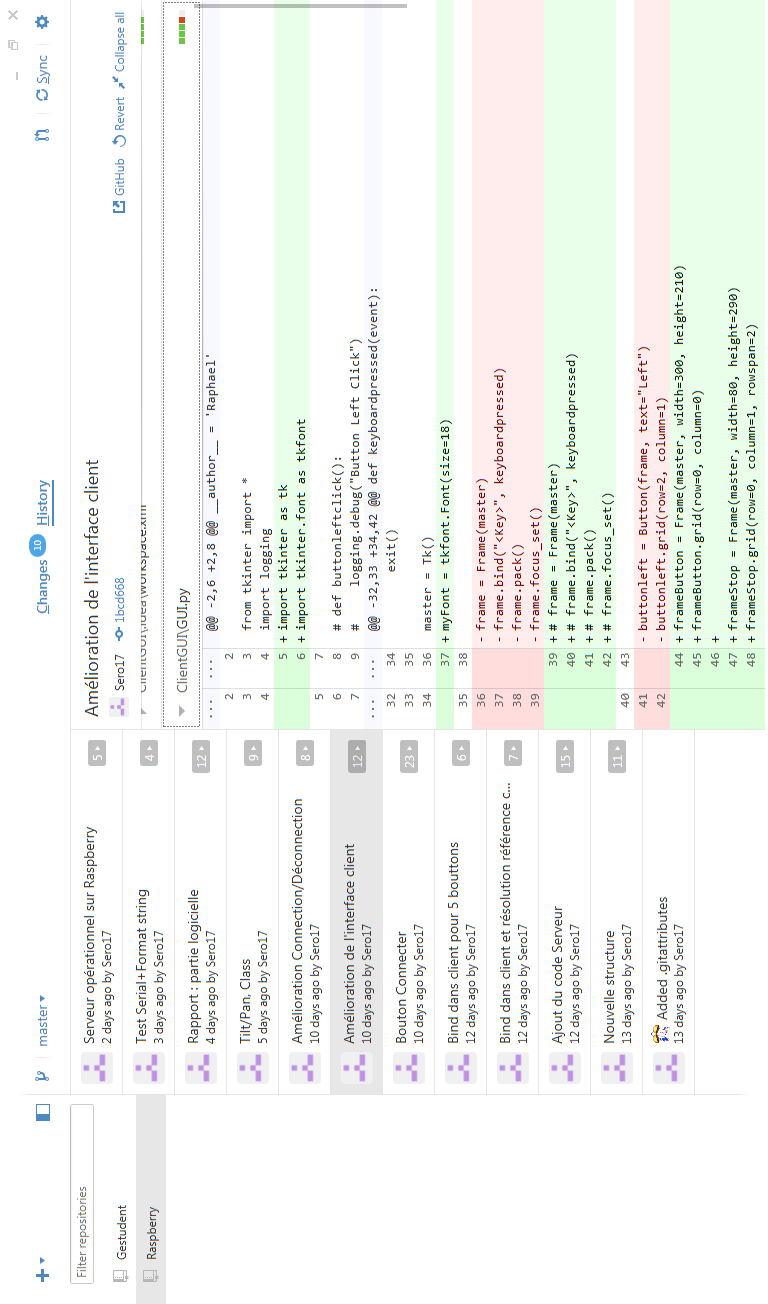
\includegraphics[scale=0.7]{images/GitHub.png}
\caption{Interface de GitHub sous Windows}
\label{GitHub}
\end{figure}

\end{itemize}

\chapter{Implémentation}

\section{Le premier robot}

Nous avions , dans un premiers temps, travaillé avec le Raspberry pi B+ et un contrôleur DC (DRV8833) pouvant gérer deux moteurs (1.2 A , 2.7-10.8 V ). Cette solution, peut couteuse, nous a permis de travailler avec les pins GPIO du Raspberry.

Nos moteurs fonctionnaient avec une tension de 5 V, et étaient directement alimentés par ces pins. Nous avons beaucoup travaillé sur la partie électronique afin d'assembler au mieux un robot. Nous avions d'abord pensé implémenter directement dans le code l'envoi de signaux PWM dans les ports GPIO, avec une boucle dans le programme qui se répète toutes les 50 millisecondes et qui, selon les commandes envoyées, permet de faire avancer, tourner ou reculer le robot.

Mais dans nos recherches, nous nous sommes aperçus que des librairies existaient déjà, et permettaient d'envoyer des signaux avec une seule commande, qui prenaient comme paramètre la vitesse relative des moteurs (100\% pour faire tourner le moteur à pleine vitesse vers l'avant, par exemple) 

Néanmoins, la qualité du matériel en notre possession n'était pas optimale : nous n'arrivions pas a fixer correctement les roues sur les axes des moteurs, et nous avons grillé le contrôleur DC lors de nos manipulations.

\begin{figure}[hf!]
\center
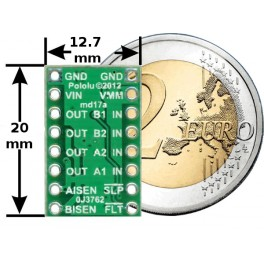
\includegraphics[scale=0.5]{images/y.jpg}
\caption{Contrôleur DRV8833}
\label{GitHub}
\end{figure}

Nous avons réalisé à ce moment l'importance d'une bonne organisation de notre travail : nous avons opté pour une réalisation du projet étape par étape : c'est-à-dire que pour chaque chose à faire, on la découpe en petites tâches "plus simples". Cette méthode présente deux avantages : on voit notre progression, car chaque étape est un pas vers la solution définitive, et si on rencontre un problème, on peut revenir à une étape antérieure qu'on sait fonctionnelle.

\section{Construction du second robot}

%Nous avons donc pris l'initiative de changer pour un kit qui nous permettrait de gagner du temps sur la partie électronique en utilisant une carte Arduino pour commander les moteurs, et surtout qui est  ayant des roues et un chassis adapté à nos envies.
Nous avons donc pris l'initiative de changer pour un kit qui nous permet d'avoir des composants compatibles entre eux, et de meilleure qualité.
%Les servo-moteurs étant géré par le raspberry afin de pouvoir jouer avec la caméra.
Les moteurs sont donc directement relié aux pins de la carte Arduino, elle-même reliée au Raspberry avec un câble USB.
L'ensemble du matériel utilisé est décrit en détail au chapitre \ref{Matériel}.

\section{PWM}

Les signaux PWM (Pulse Width Modulation) sont une technique qui nous permet d'obtenir une réponse analogique à partir d'un système fonctionnant en tout ou rien (système discret). Ce sont donc des ondes carrées dont le rapport de la largeur sur chaque période nous donne, dans ce cas-ci, la valeur de notre vitesse.
La largeur de pulsation correspond au laps de temps au cours duquel le système a la valeur 1 (5 V). Cette largeur rapportée sur l'entièreté de la période, nous donne le pourcentage d'activité, le Duty Cycle.

\begin{figure}[hf!]
\center
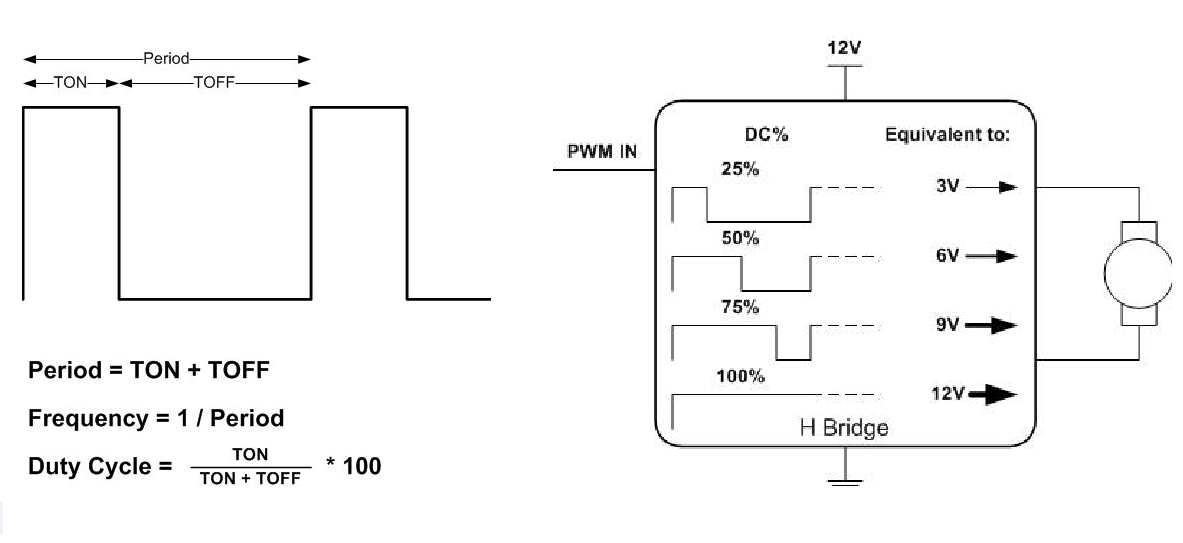
\includegraphics[scale=0.4]{images/PWM/totzal.png}
\caption{Principe des signaux PWM}
\label{GitHub}
\end{figure}

\section{Socket}

Pour notre robot, la création d'une connection Socket entre un PC et un Raspberry était nécessaire.

La première étape est de créer une connection entre un PC et ce même PC. Nous avons trouvé plusieurs exemples sur internet qui fonctionnent. Mais nous avons voulu aller plus loin pour cette étape : 

\bigbreak

\begin{itemize}
\item Ne pas envoyer une chaîne de caractère directement du code, mais la demander à l'utilisateur.
\item Traiter la chaîne reçue sur l'autre programme, simplement l'afficher, afficher le premier caractère, ou si on envoie un nombre (envoyé sous forme de chaîne), récupérer ce nombre et effectuer une opération mathématique simple.
\item Envoyer une chaîne (n'importe quoi, cela n'a pas d'importance), puis dès que l'autre programme reçoit cette chaîne, renvoyer une autre chaîne.
\item Sur le PC, gérer avec Python les dates.
\end{itemize}

\bigbreak

Ainsi avec quelques étapes "faciles", on peut affirmer :

\bigbreak

\begin{itemize}
\item On sait ouvrir une connection,
\item On peut envoyer n'importe quelle information "simple" (types de données courants),
\item On sait la récupérer et la traiter de l'autre coté,
\item On sait estimer le temps que ça prend pour l'envoi (lors de nos tests, l'aller-retour prenait environ 0.7 secondes).
\item On sait comment fonctionne le code, car au lieu de recopier bêtement d'internet, on l'a modifié en cherchant à comprendre son fonctionnement.
\end{itemize}

\bigbreak

Ensuite, nous avons répété les mêmes processus entre un PC (sous Windows) et une machine virtuelle (sous Debian). Ces étapes sont normalement immédiates, puisque tous les codes ont déjà été écrits à l'étape précédente.

\bigbreak

Enfin, nous avons refait la même chose entre le PC et le Raspberry. Nous avons dès lors atteint notre objectif, à savoir envoyer des instructions depuis le PC, vers le Raspberry.

\chapter{Qui a fait quoi}

Raphaël

Recherches sur connection socket

Programme client, interface, programme serveur sur raspberry, connection serial avec arduino
Backup régulier des codes sur GitHub, ...

\chapter{Conclusion}

Difficultés rencontrées, limitations, améliorations possibles, ...

\appendix

\chapter{Procédure d'installation}

\section{Installation de Raspbian sur le Raspberry Pi}

Voici la procédure à suivre pour installer Raspbian sur le Raspberry :

\begin{itemize}
\item Téléchargez NOOBS sur \,\url{https://www.raspberrypi.org/downloads/}, et extrayez les fichiers du zip.

\item Formatez la carte SD (avec \,\url{https://www.sdcard.org/downloads/formatter_4/}). Sélectionnez la carte SD et dans les options choisissez \textit{FORMAT SIZE ADJUSTMENT ON}, puis cliquez sur \verb=Format=.

\item Copiez les fichiers extraits de NOOBS sur la carte SD, puis éjectez la carte et insérez-la dans le Raspberry Pi.

\item Connectez le Raspberry à un écran avec un câble HDMI, et connectez aussi un clavier et une souris sur les ports USB (un récepteur sans fil convient aussi).

\item Alimentez le Raspberry. Attention il est déconseillé de brancher/débrancher des câbles lorsque le Raspberry est sous tension. Si vous souhaitez changer l'écran ou un autre périphérique, éteignez d'abord le Raspberry et débranchez-le.

\item Sélectionnez Rasbian comme OS et la langue, ainsi que la configuration du clavier, et cliquez sur \textit{Installer}.

\item Après l'installation (compter environ 25 minutes), redémarrez le Raspberry Pi.

\item Dans les options proposées, choisissez \textit{Enable Boot to Desktop/Scratch}, et \textit{Desktop Log in as user 'pi'}. Ensuite dans \textit{Advanced Options}, choisissez \textit{SSH}, et \textit{Enable}. Allez sur \textit{Finish} (avec Tabulation) et redémarrez le Raspberry.

\item Si vous utilisez un écran avec un câble VGA et un adaptateur, il faut modifier \url{\boot\config.txt}. Il faut décommenter ou ajouter les lignes suivantes : 
\begin{verbatimtab}[3]
hdmi_force_hotplug=1
hdmi_group=2
hdmi_mode=69
hdmi_drive=2
\end{verbatimtab}
Le numéro 69 correspond à une résolution d'écran de 1920x1200, et une fréquence de 60 hz. Pour voir quel numéro correspond, voir \url{https://www.raspberrypi.org/documentation/configuration/config-txt.md}\, .

\item Configurez le WiFi (voir section suivante), et mettez à jour le système en entrant ces deux commandes :

\bigbreak
\begin{verbatimtab}[3]
sudo apt-get update
sudo apt-get upgrade
\end{verbatimtab}
\bigbreak

\end{itemize}



\section{Configurer le WiFi sur le Raspberry Pi}

Nous allons configurer le Raspberry pour se connecter au routeur, et lui assigner une IP fixe.

\begin{itemize}
\item Lorsque le Raspberry est hors tension, insérez la clé WiFi dans un port USB.
%\item Dans un terminal, entrez la commande \,\verb=ifconfig= pour récupérer ceci :
%
%\bigbreak
%\begin{verbatimtab}[3]
%wlan0	Link encap:Ethernet	HWaddr c4:a8:1d:7c:0b:60
%inet adr:192.168.1.104	Bcast:192.168.1.255	Masque:255.255.255.0
%\end{verbatimtab}
%\bigbreak
%
%\item Entrez ensuite \,\verb=sudo route -n=  :
%
%\bigbreak
%\begin{tabular}{lll}
%\verb=Destination= & \verb=Passerelle= & \verb=Genmask= \\ 
%\verb=0.0.0.0= & \verb=192.168.1.1= & \verb=0.0.0.0= \\ 
%\verb=192.168.1.0= & \verb=0.0.0.0= & \verb=255.255.255.0=\\ 
%\end{tabular}
%\bigbreak

\item Toutes les informations concernant le réseau peuvent être retrouvées grâce à un autre appareil connecté à ce réseau : entrez dans un terminal ces deux commandes :

\bigbreak
\begin{verbatimtab}[3]
sudo route -n
ifconfig
\end{verbatimtab}
\bigbreak

\item On édite un premier fichier de configuration : entrez cette commande : 

\bigbreak
\begin{verbatimtab}[3]
sudo nano /etc/wpa_supplicant/wpa_supplicant.conf
\end{verbatimtab}
\bigbreak

Ajoutez les paramètres du réseau Wi-Fi, et sauvegardez :

\begin{verbatimtab}[3]
network={
	ssid="<SSID du réseau local>"
	psk="<Clé de sécurité>"
	proto=RSN
	key_mgmt=WPA-PSK
	paiwise=CCMP
	auth_alg=OPEN
}
\end{verbatimtab}

\item On édite un autre fichier : entrez cette commande : 

\bigbreak
\begin{verbatimtab}[3]
sudo nano /etc/network/interfaces
\end{verbatimtab}
\bigbreak

Ajoutez les paramètres du réseau Wi-Fi, et sauvegardez :

\bigbreak
\begin{verbatimtab}[3]
auto lo

iface lo inet loopback
iface eth0 inet dhcp

allow-hotplug wlan0
auto wlan0

iface wlan0 inet static
address 192.168.1.50
netmask 255.255.255.0
broadcast 192.168.1.255
gateway 192.168.1.1
wpa-conf /etc/wpa_supplicant/wpa_supplicant.conf
iface default inet dhcp
\end{verbatimtab}
\bigbreak

L'adresse 192.168.1.50 est l'adresse IP que j'ai choisie pour le Raspberry. Il faut choisir une adresse en dehors de la plage d'adresse réservée pour le dhcp.

\item Réinitialisez le réseau avec ces deux commandes, ou redémarrez le Raspberry.

\bigbreak
\begin{verbatimtab}[3]
sudo ifdown wlan0
sudo ifup wlan0
\end{verbatimtab}
\bigbreak
\end{itemize}

\end{document}

